\documentclass[aspectratio=149]{beamer}

\usepackage{bm}
\usetheme{metropolis}           % Use metropolis theme
\title{Variational Linearized Laplace Approximation for Bayesian Deep Learning}
\date{\today}
\author{Luis Antonio Ortega Andrés}
\institute{Autonomous University of Madrid}

\NeedsTeXFormat{LaTeX2e}
\usepackage{amsfonts}       % blackboard math symbols
\usepackage{amssymb,amsmath,amsthm}

\usepackage{braket}

\usefonttheme{professionalfonts} % required for mathspec
\usepackage{mathspec}
\setsansfont[BoldFont={Fira Sans}]{Fira Sans Light}
\usepackage[natbib=true, backend=biber, style=authoryear-icomp, useprefix=true]{biblatex}
\addbibresource{slidesrefs.bib}

\begin{document}
  \maketitle


    {\setbeamercolor{background canvas}{bg=white}
      \begin{frame}{}
        \begin{figure}
            \centering
            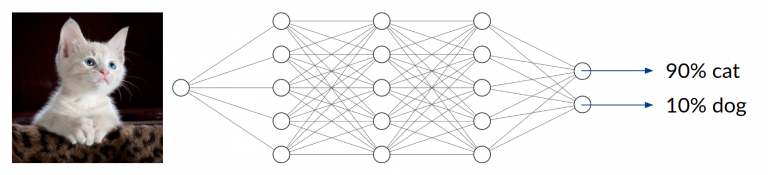
\includegraphics[width = 0.8\textwidth]{slides_imgs/Bildschirmfoto-vom-2019-10-01-11-03-08-768x175.png}
            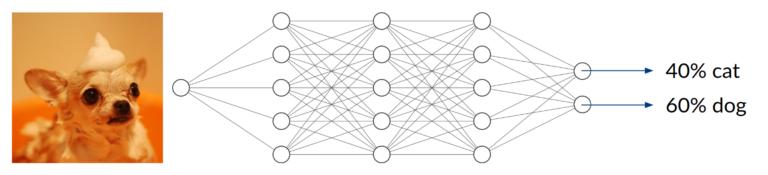
\includegraphics[width = 0.8\textwidth]{slides_imgs/uncertainty-quantification-dog-768x175.png}
            \label{fig:my_label}
        \end{figure}
    \end{frame}}
    
    {\setbeamercolor{background canvas}{bg=white}
      \begin{frame}{}
        \begin{figure}
            \centering
            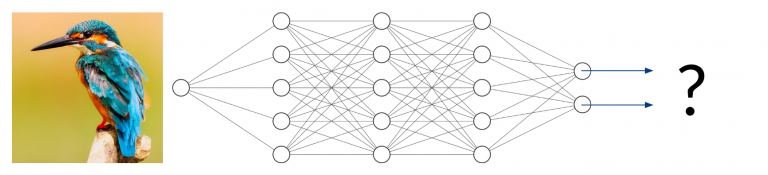
\includegraphics[width = 0.8\textwidth]{slides_imgs/Bildschirmfoto-vom-2019-10-01-11-03-18-768x175.png}
            \label{fig:my_label}
        \end{figure}
    
        \onslide<2>{\textbf{Deep learning methods are unable to quantify the uncertainty of their predictions!}}
    \end{frame}}
    
    {\setbeamercolor{background canvas}{bg=white}
      \begin{frame}{}
      \textbf{Straight-forward solution}: Using a Bayesian model.
        \begin{figure}
            \centering
            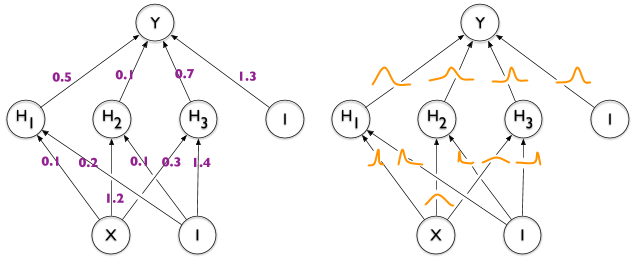
\includegraphics[width = 0.8\textwidth]{slides_imgs/Bayesian-Neural-Network.png}
            \label{fig:my_label}
        \end{figure}
    \end{frame}}

    \begin{frame}
        Making predictions requires the posterior over the parameters of the model \(\bm{\theta}\):
        \[
            P(y^\star | \mathbf{x}^\star, \mathcal{D}) = \int P(y^\star | \mathbf{x}^\star, \bm{\theta}) P(\bm{\theta} | \mathcal{D}) \ d\bm{\theta}
        \]
        where \( P(\bm{\theta} | \mathcal{D}) \) is \textbf{intractable for complex models}.
    \end{frame}


    \begin{frame}
        \begin{center}
            Approximate  \( P(\bm{\theta} | \mathcal{D}) \) by something simpler \(Q(\bm{\theta})\).
            \onslide<2>
            {
                \[
                    \Bigg\Downarrow
                \]
                \textbf{Poor performance of the model in many cases.}
            }
        \end{center}
    \end{frame}


    \section{Laplace Approximation for Deep Learning}

    {\setbeamercolor{background canvas}{bg=white} 
        \begin{frame}
        \begin{center}
            \begin{tabular}{ccc}
                Deep Model & & Dataset\\
                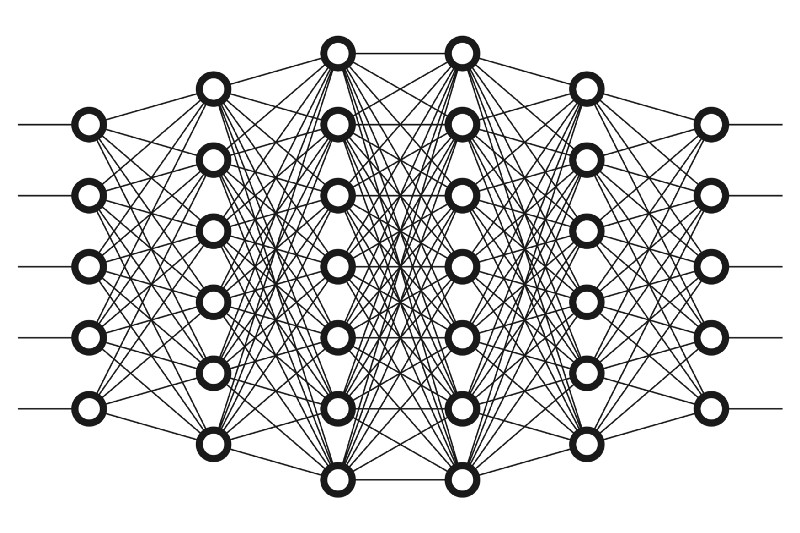
\includegraphics[width=0.3\textwidth]{slides_imgs/deep_model.jpeg} & &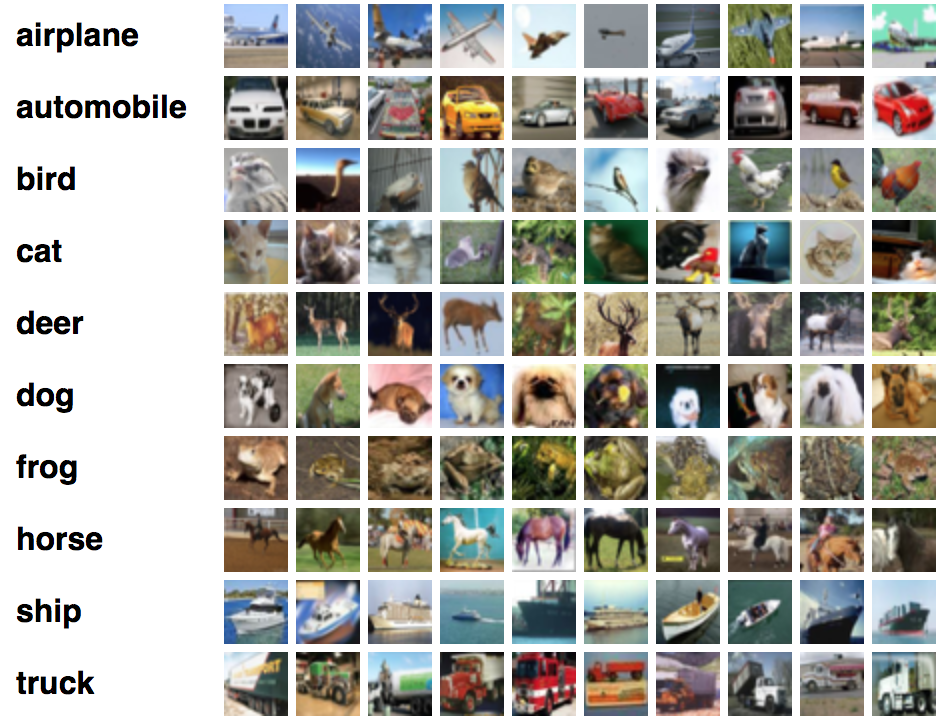
\includegraphics[width=0.3\textwidth]{slides_imgs/dataset.png}  \\
                & \Big\Downarrow &
            \end{tabular}
        \end{center}
        \begin{center}
            Optimal parameter \(\hat{\bm{\theta}}\) using deep learning techniques.\\
        \end{center}
        \end{frame}
    }

    \begin{frame}
        Given the optimal parameters \(\hat{\bm{\theta}}\), we aim to make \textbf{uncertainty estimation} on the pre-trained model.

        \only<1>{\vspace*{6.5cm}}

        \only<2,3,4>{\textbf{Laplace approximation} (LA) of \(P(\bm{\theta}|\mathcal{D})\) centered on \(\hat{\bm{\theta}}\) as
        \[
        P(\bm{\theta}|\mathcal{D}) \approx Q(\bm{\theta}) = \mathcal{N}(\bm{\theta} | \hat{\bm{\theta}}, \bm{\Sigma})
        \]
        where}\only<2>{
        \[
            \bm{\Sigma}^{-1} = -\nabla^2_{\bm{\theta} \bm{\theta}} \log P(\bm{\theta} |\mathcal{D})_{|\bm{\theta} = \hat{\bm{\theta}} } = -\nabla^2_{\bm{\theta} \bm{\theta}} (\log P(\mathcal{D}|\bm{\theta}) + \log P(\bm{\theta}))_{|\bm{\theta} = \hat{\bm{\theta}}}
        \]
        \vspace*{2cm}
        }
        \only<3>{
        \[
            \bm{\Sigma}^{-1} = -\nabla^2_{\bm{\theta} \bm{\theta}} \log P(\bm{\theta} |\mathcal{D})_{|\bm{\theta} = \hat{\bm{\theta}} } = -\nabla^2_{\bm{\theta} \bm{\theta}} \log P(\mathcal{D}|\bm{\theta}) + {\color{red}\frac{1}{\sigma_0^2}\bm{I}_P}
        \]
        \vspace*{2cm}
        }\only<4>{applying the \textbf{\alert{generalized Gauss-Newton matrix approximation}}
        \[
            \bm{\Sigma}^{-1} \approx \tilde{\bm{\Sigma}}^{-1}  = \sum_{n=1}^{N} \mathcal{J}_{\hat{\bm{\theta}}}(\mathbf{x}_n) \Lambda(\mathbf{x}_n, y_n) \mathcal{J}_{\hat{\bm{\theta}}}(\mathbf{x}_n)^T + \frac{1}{\sigma_0^2}\bm{I}_P\,.
        \]
        with 
        \[
            \mathcal{J}_{\hat{\bm{\theta}}}(\mathbf{x}_n) = \nabla_{\bm{\theta}} g(\mathbf{x}_n, \bm{\theta})_{|\bm{\theta} = \hat{\bm{\theta}}} \quad
            \Lambda(\mathbf{x}_n, y_n) = -\nabla^2_{\mathbf g \mathbf g} \log P(y_n|\mathbf g)_{|\mathbf g = g(\mathbf x_n, \hat{\bm{\theta}})}
        \]
        }
    \end{frame}

    \begin{frame}
        \begin{center}
            \textbf{The Laplace approximation of the deep model has poor performance}.
            
            \onslide<2->{
            $\Big \Downarrow$
            
            There is a shift between the posterior and the predictive distribution. 
            \[
                Q(\bm{\theta}) = \mathcal{N}(\bm{\theta} | \hat{\bm{\theta}}, \tilde{\bm{\Sigma}}) \quad  P(y^\star | \mathbf{x}^\star, \mathcal{D}) \approx \mathbb{E}_{Q(\bm{\theta})} \left[P(y^\star | {\only<3>{\color{red}}g}(\mathbf{x}^\star, \bm{\theta}))\right]
            \]
            }
            \onslide<3->{
            The GGN approximation, is the true posterior of a linearized model
            \[
                g^{lin}(\mathbf{x}, \bm{\theta}) = g(\mathbf{x}, \hat{\bm{\theta})} + \mathcal{J}_{\hat{\bm{\theta}}}(\mathbf{x}_n) ^T(\bm{\theta} - \hat{\bm{\theta}})
            \]
            Which means, that predictions should be made over the linearized model:
            \[
                  P(y^\star | \mathbf{x}^\star, \mathcal{D}) \approx \mathbb{E}_{Q(\bm{\theta})} \left[P(y^\star | {\only<3>{\color{red}}g^{lin}}(\mathbf{x}^\star, \bm{\theta}))\right]
            \]
            }
        \end{center}
    \end{frame}

    \begin{frame}
        \begin{center}
            The \textbf{linearized Laplace approximation} (LLA) is equivalent to a \textbf{Gaussian Process}.
            \vspace{1cm}

            \onslide<2->{
            Prior distribution
            \[
                P(\bm{\theta}) = \mathcal{N}(\bm{m}, \bm{S})
            \]
            }
            \onslide<3->{
            $\Downarrow$
            
            Gaussian Process
            \begin{align*}
                m(\mathbf x) &= g^{lin}(\mathbf x, \bm{m})\\
                K(\mathbf x, \mathbf x') &= \mathcal{J}_{\hat{\bm{\theta}}}(\mathbf{x})^T \bm{S} \mathcal{J}_{\hat{\bm{\theta}}}(\mathbf{x}' )
            \end{align*}
            }
        \end{center}
    \end{frame}

    \begin{frame}
        \begin{center}
        Using LLA approximate posterior 
            \[
                Q(\bm{\theta}) = \mathcal{N}(\hat{\bm{\theta}},\tilde{\bm{\Sigma}})
            \]
            $\Downarrow$
            
            Gaussian Process
            \[
                m^\star(\mathbf x) = g^{lin}(\mathbf x, \hat{\bm{\theta}})
            \]
            \[
                K^\star(\mathbf x, \mathbf x') = \sigma_0^2\left( \kappa(\mathbf{x}, \mathbf{x}') - \kappa(\mathbf{x}, \mathbf{X})\left(  \frac{1}{\sigma_0^2} \bm{\Lambda}_{\mathbf{X}, \mathbf{y}}^{-1} + \kappa(\mathbf{X}, \mathbf{X}) \right)^{-1} \kappa(\mathbf{X}, \mathbf{x}' )\right)\,.
            \]
            where \(\kappa(\mathbf{x}, \mathbf{x}') = \mathcal{J}_{\hat{\bm{\theta}}}(\mathbf{x})^T\mathcal{J}_{\hat{\bm{\theta}}}(\mathbf{x}' )\).
        \end{center}
    \end{frame}

    \begin{frame}
        \textbf{Main idea}: Approximate the exact GP posterior using a sparse approach with inducing points.

        \textbf{Main inconvenience}: Using a sparse GP \textbf{changes the predictive mean}, loosing the pre-trained solution.

        \textbf{Solution}: Use a Generalized Sparse GP in the RKHS.
    \end{frame}

    \begin{frame}{Dual representation of Gaussian Processes}

        An RKHS \(\mathcal{H}\) is a Hilbert space of functions satisfying the reproducing property: \(\forall \mathbf{x} \in \mathcal{X} \ \exists \phi_{\mathbf{x}} \in \mathcal{H}\) such that \(\forall f \in \mathcal{H}, f(\mathbf{x}) = \braket{\phi_{\mathbf{x}}, f} \).

        \onslide<2->{
        A \textbf{Gaussian process} \(\mathcal{GP}(m, K)\) has a dual representation in a RKHS as: there exists \(\mu \in \mathcal{H}\) and a linear semi-definite positive operator \(\Sigma:\mathcal{H} \to \mathcal{H}\) such that, for any \(\mathbf{x}, \mathbf{x}' \in \mathcal{X}\), \(\exists \phi_{\mathbf{x}}, \phi_{\mathbf{x}'}\), verifying
        \[
            m(\mathbf{x}) = \braket{\phi_{\mathbf{x}}, \mu}, \quad K(\mathbf{x}, \mathbf{x}') = \braket{\phi_{\mathbf{x}}, \Sigma(\phi_{\mathbf{x}'})}
        \]}
        \onslide<3->{As an abuse of notation, we write \(f \sim \mathcal{N}(\mu, \Sigma)\), which is a Gaussian measure in the RKHS.
        }
    \end{frame}

    \begin{frame}
        \textbf{Theorem} \citep{cheng2016incremental}. Using a sparse GP approximation with variational distribution \(q(\mathbf{f}, \mathbf{u}) = p(\mathbf{f}|\mathbf{u})q(\mathbf{u})\) is equivalent to restricting the mean and covariance functions of the dual representation in the RKHS to
        \[
            \tilde{\mu} = \Phi_{\mathbf{Z}}(\bm{a}) \quad \text{and} \quad \tilde{\Sigma} = I + \Phi_{\mathbf{Z}}\bm{A}\Phi_{\mathbf{Z}}^T\,,
        \]
        where \(\Phi_{\mathbf{Z}}: \mathbb{R}^M \to \mathcal{H} \) is defined as \(\Phi_{\mathbf{Z}}(\bm{a}) = \sum_{m=1}^{M} a_m \phi_{\mathbf{z}_m}\),  \(\bm{a} \in \mathbb{R}^M\) and \(\Phi_{\mathbf{Z}}\bm{A}\Phi_{\mathbf{Z}}^T= \sum_{i=1}^{M}\sum_{j=1}^M\phi_{\mathbf{z}_i} A_{i,j} \phi_{\mathbf{z}_j}^T\), \(\bm{A} \in \mathbb{R}^{M\times M}\) such that \(\tilde{\Sigma} \geq 0\).
    \end{frame}

    \begin{frame}
        \textbf{Theorem} \citep{cheng2016incremental}. Using a sparse GP approximation with variational distribution \(q(\mathbf{f}, \mathbf{u}) = p(\mathbf{f}|\mathbf{u})q(\mathbf{u})\) is equivalent to restricting the mean and covariance functions of the dual representation in the RKHS to
        \[
            \tilde{\mu} = \Phi_{\color{red}\mathbf{Z}_\alpha}(\bm{a}) \quad \text{and} \quad \tilde{\Sigma} = I + \Phi_{\color{red}\mathbf{Z}_\beta }\bm{A}\Phi_{\color{red}\mathbf{Z}_\beta}^T\,,
        \]
        where \(\Phi_{\mathbf{Z}}: \mathbb{R}^M \to \mathcal{H} \) is defined as \(\Phi_{\color{red}\mathbf{Z}_\alpha }(\bm{a}) = \sum_{m=1}^{M} a_m \phi_{\mathbf{z}_m}\),  \(\bm{a} \in \mathbb{R}^M\) and \(\Phi_{\color{red}\mathbf{Z}_\beta }\bm{A}\Phi_{\color{red}\mathbf{Z}_\beta }^T= \sum_{i=1}^{M}\sum_{j=1}^M\phi_{\mathbf{z}_i} A_{i,j} \phi_{\mathbf{z}_j}^T\), \(\bm{A} \in \mathbb{R}^{M\times M}\) such that \(\tilde{\Sigma} \geq 0\).
    \end{frame}

     {\setbeamercolor{background canvas}{bg=white}\begin{frame}

        \begin{figure}
            \centering
            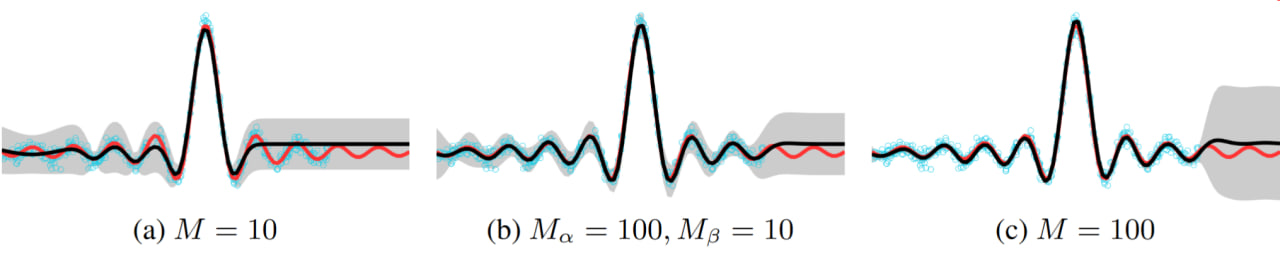
\includegraphics[width = 0.96\textwidth]{slides_imgs/decoupled.jpg}
        \end{figure}
        Comparison between models with shared and decoupled basis.
        
        \begin{itemize}
            \item (a)(c) denote the models with shared basis of size \(M\).
            \item (b) denotes the model of decoupled basis with size (\(M_\alpha, M_\beta\)).
        \end{itemize} 
    \end{frame}}

    \begin{frame}

        For any function \(t \in \mathcal{H}\), and \(\epsilon > 0\), there exists a set of points \(\mathbf{Z}_\alpha \subset \mathcal{X}\) and coefficients \(\bm{a}\), such that
        \[
            d_{\mathcal{H}}(t, h_\epsilon) \leq \epsilon, \text{ with } h_\epsilon = \Phi_{\mathbf{Z}_\alpha}(\bm{a})\,.
        \]

        \onslide<2->{We can fit the mean of the posterior distribution of the sparse decoupled GP to any function in the Hilbert space (\(g(\cdot, \hat{\bm{\theta}})\)).}

        \onslide<3->{If \(g(\cdot, \hat{\bm{\theta}}) \not \in \mathcal{H}\), we can use that \(\mathcal{H}\) is dense in the span of the Gaussian Process. 
        }
    \end{frame}

    \begin{frame}
        \textbf{Proposition.} If \(g(\cdot, \hat{\bm{\theta}}) \in \mathcal{H}\), \(\forall \epsilon > 0\), there exists a set of \(M_\alpha\) inducing points \(\mathbf{Z}_{\alpha} \subset \mathcal{X}\) and \(\bm{a} \in \mathbb{R}^{M_\alpha}\) such that the dual representation in the RKHS of the corresponding sparse Gaussian process defined by
        \[
            \tilde{\mu} = \Phi_{\mathbf{Z}_{\alpha}}(\bm{a}) \quad \text{and} \quad \tilde{\Sigma} = (I + \Phi_{\mathbf{Z}_{\beta}}\bm{A}\Phi_{\mathbf{Z}_{\beta}}^T)^{-1}\,,
        \]
        corresponds to a posterior approximation \(\mathcal{GP}(m^\star, K^\star)\) with mean and covariance functions defined as
        \[
            \begin{aligned}
                m^{\star}(\mathbf{x}) &= h_\epsilon(\mathbf{x})\,, \\
                K^{\star}(\mathbf{x}, \mathbf{x}') &=K(\mathbf{x}, \mathbf{x}') -  K_{\mathbf{x}, \mathbf{Z}_\beta}(\bm{A}^{-1} + K_{\mathbf{Z}_\beta})^{-1} K_{\mathbf{Z}_\beta, \mathbf{x}'}\,,
            \end{aligned}
        \]
        where \(\mathbf{Z}_{\beta} \subset \mathcal{X} \) is a set of \(M_\beta\) inducing points, \(\bm{A} \in \mathbb{R}^{M_\beta \times M_\beta}\) such that \(\tilde{\Sigma} \geq 0\) and \(h_\epsilon\) verifies \( d_{\mathcal{H}}(g(\cdot, \hat{\bm{\theta}}), h_\epsilon) \leq \epsilon\,\).
    \end{frame}

    \begin{frame}
        Optimizing the ELBO in the Hilbert space:
        \[
        \begin{aligned}
        \max_{q(f), \bm{\theta}} \mathcal{L}_{\bm{\theta}} (q(f)) &= \max_{q(f), \bm{\theta}} \int q(f) \log \frac{p_{\bm{\theta}}(y|f)p(f)}{q(f)} df \\
        &= \max_{q(f), \bm{\theta}}\mathbb{E}_q \left[ \log p_{\bm{\theta}}(y|f)\right] - \text{KL}\left(q \mid p\right)\,.
        \end{aligned}
        \]
        where
        \[
            \begin{aligned}
                \text{KL}\left(q \mid p\right) = \frac{1}{2} \bm{a}^T \bm{K}_{\alpha} \bm{a} + \frac{1}{2} \log |\bm{I} + \bm{K}_{\beta} \bm{A}| - \frac{1}{2} \text{tr}\left( \bm{K}_\beta(\bm{A}^{-1} + \bm{K}_\beta)^{-1} \right)
            \end{aligned}
        \]
    \end{frame}

    \begin{frame}{Intuitive Recap}
        \begin{enumerate}[<+->]
            \item The Linearized Laplace Approximation is equivalent to a GP.
            \item Sparse approach based on inducing points to approximate the posterior GP.
            \item Separate the inducing locations from the mean and covariance.
            \item Use ``\emph{infinite}'' inducing points for the mean. Fixing the mean to the pre-trained MAP solution.
            \item The resulting method does scale with the number of parameters and the dataset size (mini-batch optimization).
        \end{enumerate}
    \end{frame}

    \begin{frame}{ELLA}
        Another existing sparse approximation is ELLA. 

        \begin{enumerate}
            \item Approximated the kernel matrix of the full dataset using a random subset of it.
            \[  
                \hat{\mathbf X} \subset \mathbf X \implies \hat{\bm{K}} = \mathcal{J}_{\hat{\bm{\theta}}}(\hat{\mathbf{X}}) \mathcal{J}_{\hat{\bm{\theta}}}(\hat{\mathbf{X}}) ^T \approx \bm{K} = \mathcal{J}_{\hat{\bm{\theta}}}(\mathbf{X}) \mathcal{J}_{\hat{\bm{\theta}}}(\mathbf{X}) ^T 
            \]
            \item Finds eigen-decomposition of \(\hat{\bm{K}}\) to create lower-dimensional features \(\phi(\mathbf x)\).
            \item Use these features to approximate the true covariance matrix \(\bm{K}\).
            \item Requires an unique iteration over the whole training dataset.
        \end{enumerate}
    \end{frame}

    \begin{frame}{Preliminary results}
        \begin{figure}
        	\begin{center}
        	\begin{tabular}{ccc}
            {\scriptsize LLA }& {\scriptsize VaLLA }& {\scriptsize ELLA} \\
        	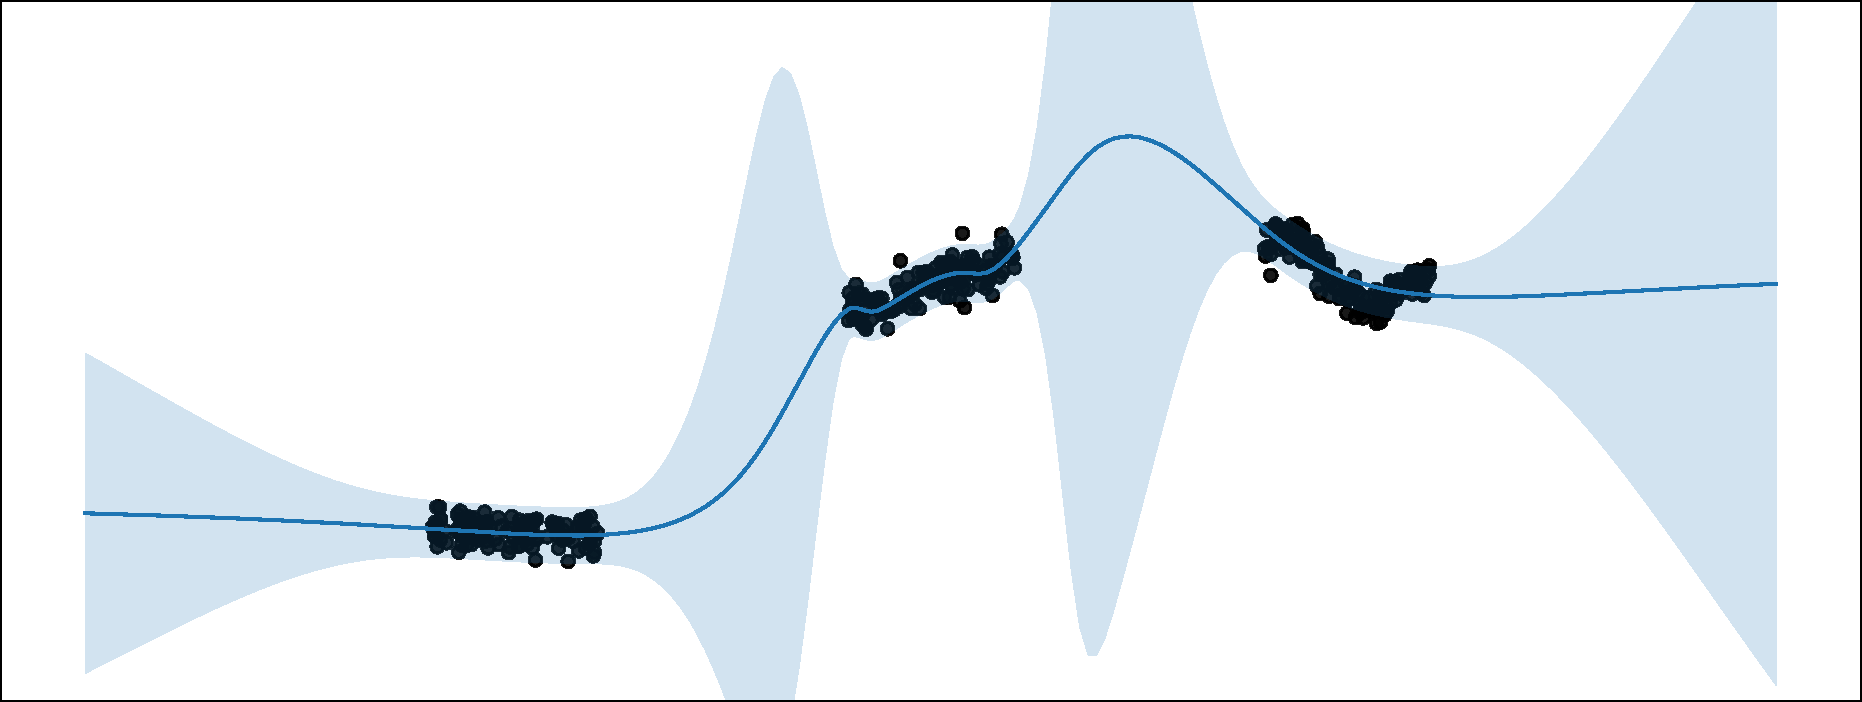
\includegraphics[width=0.30\textwidth]{imgs/LLA} & 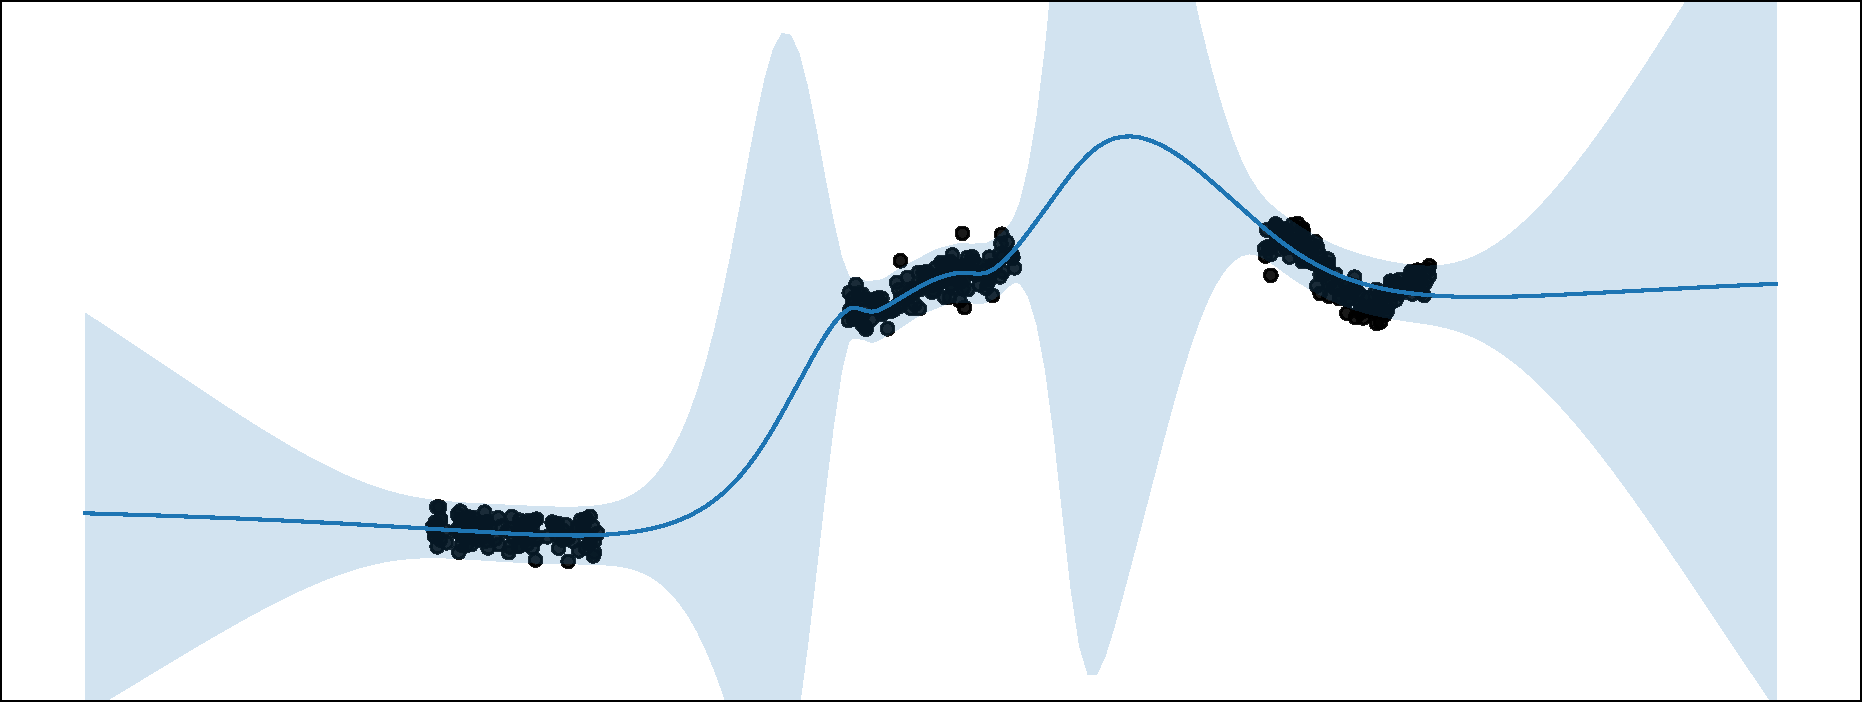
\includegraphics[width=0.30\textwidth]{imgs/VaLLA} & 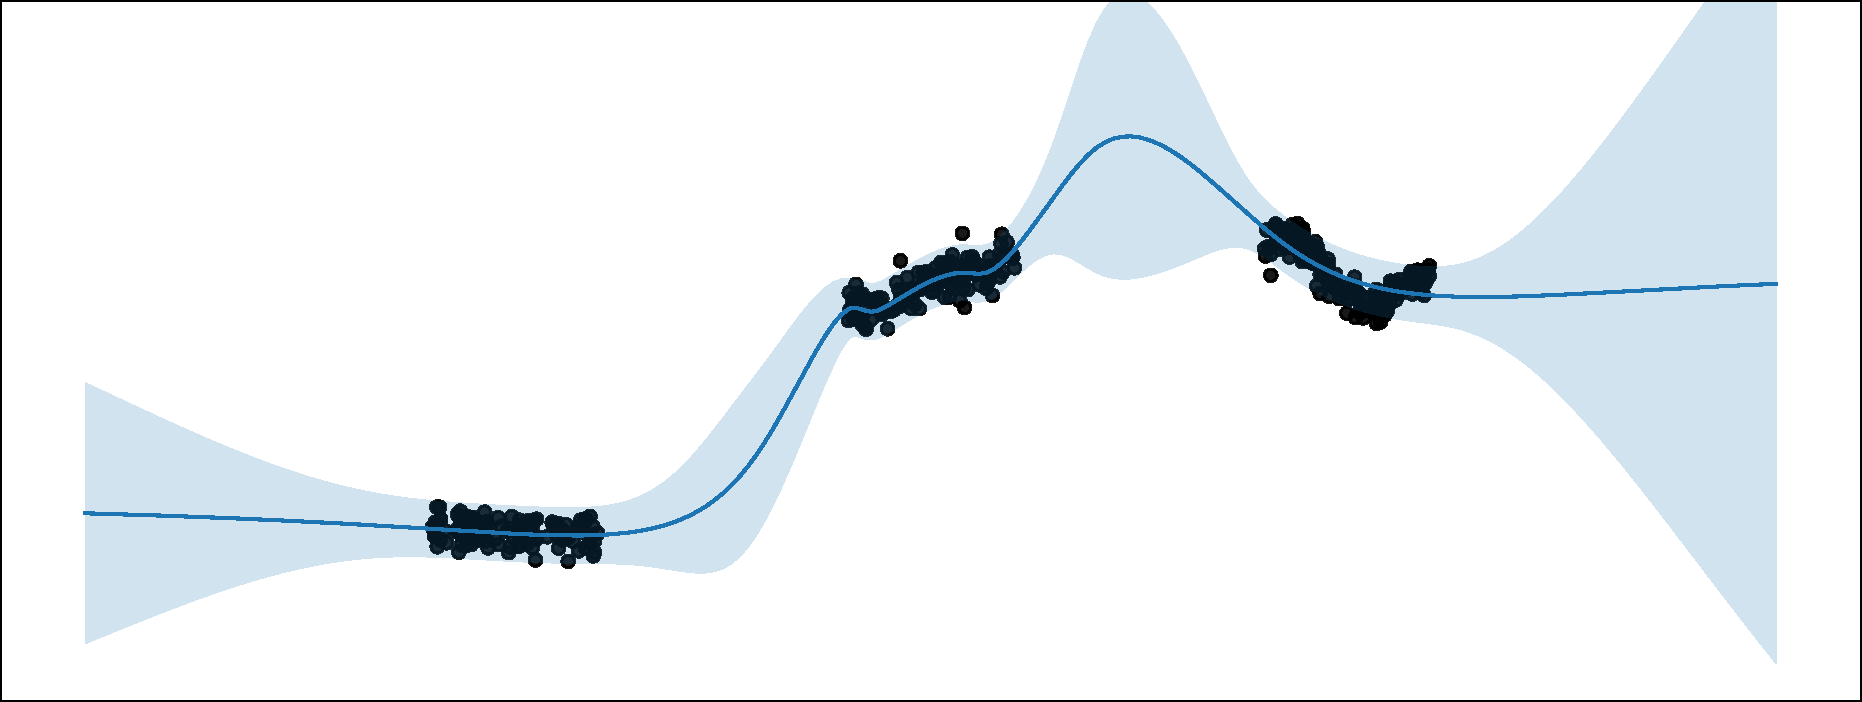
\includegraphics[width=0.30\textwidth]{imgs/ELLA.pdf} \\
            {\scriptsize Last-Layer LLA} & {\scriptsize Diagonal LLA} & {\scriptsize Kronecker LLA}\\
        	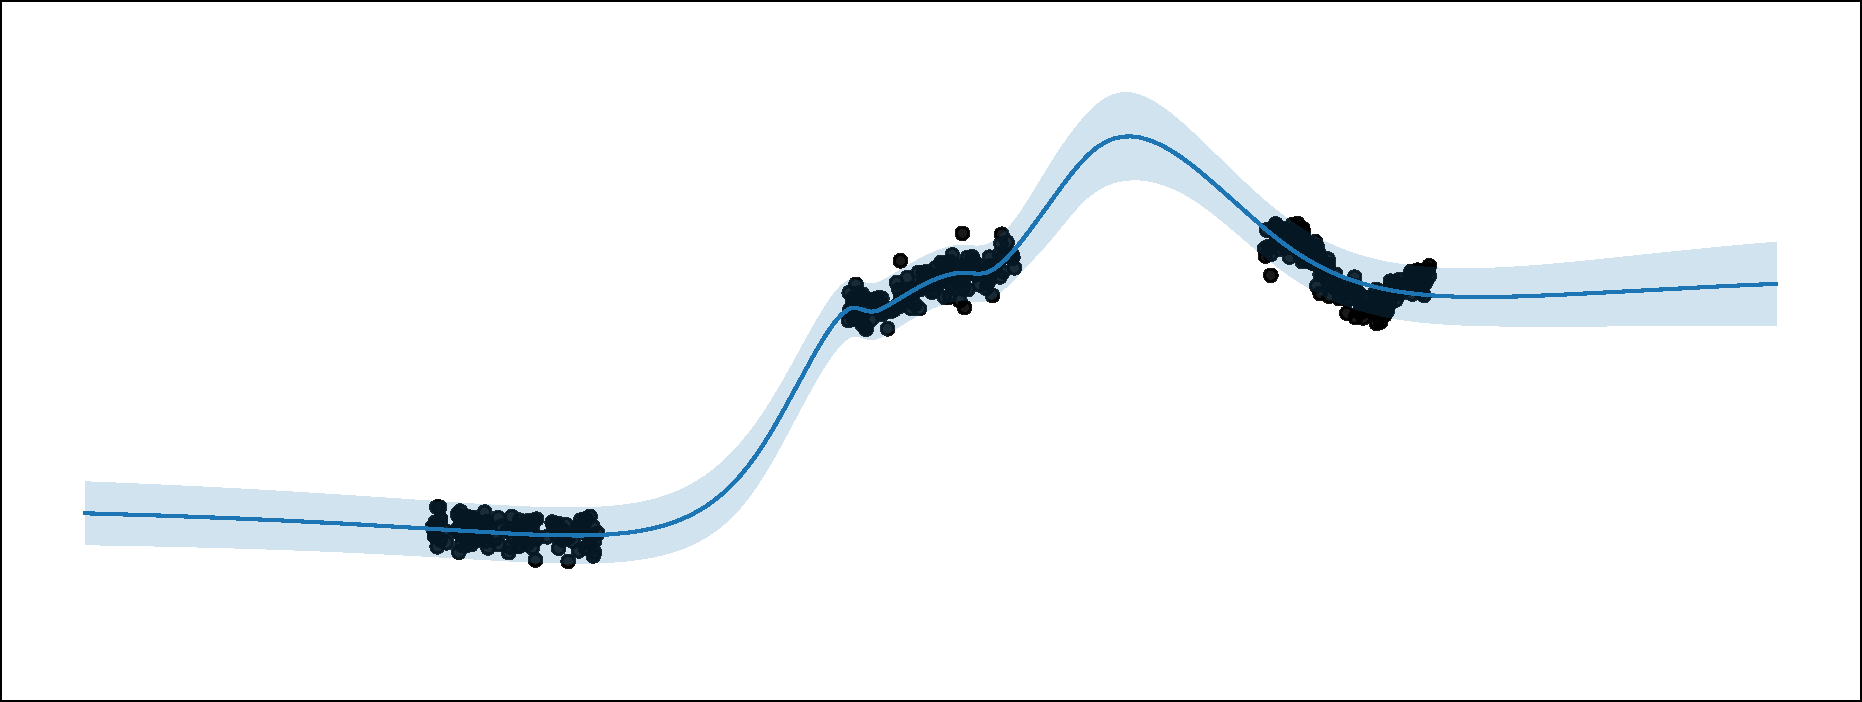
\includegraphics[width=0.30\textwidth]{imgs/LL-LLA.pdf} & 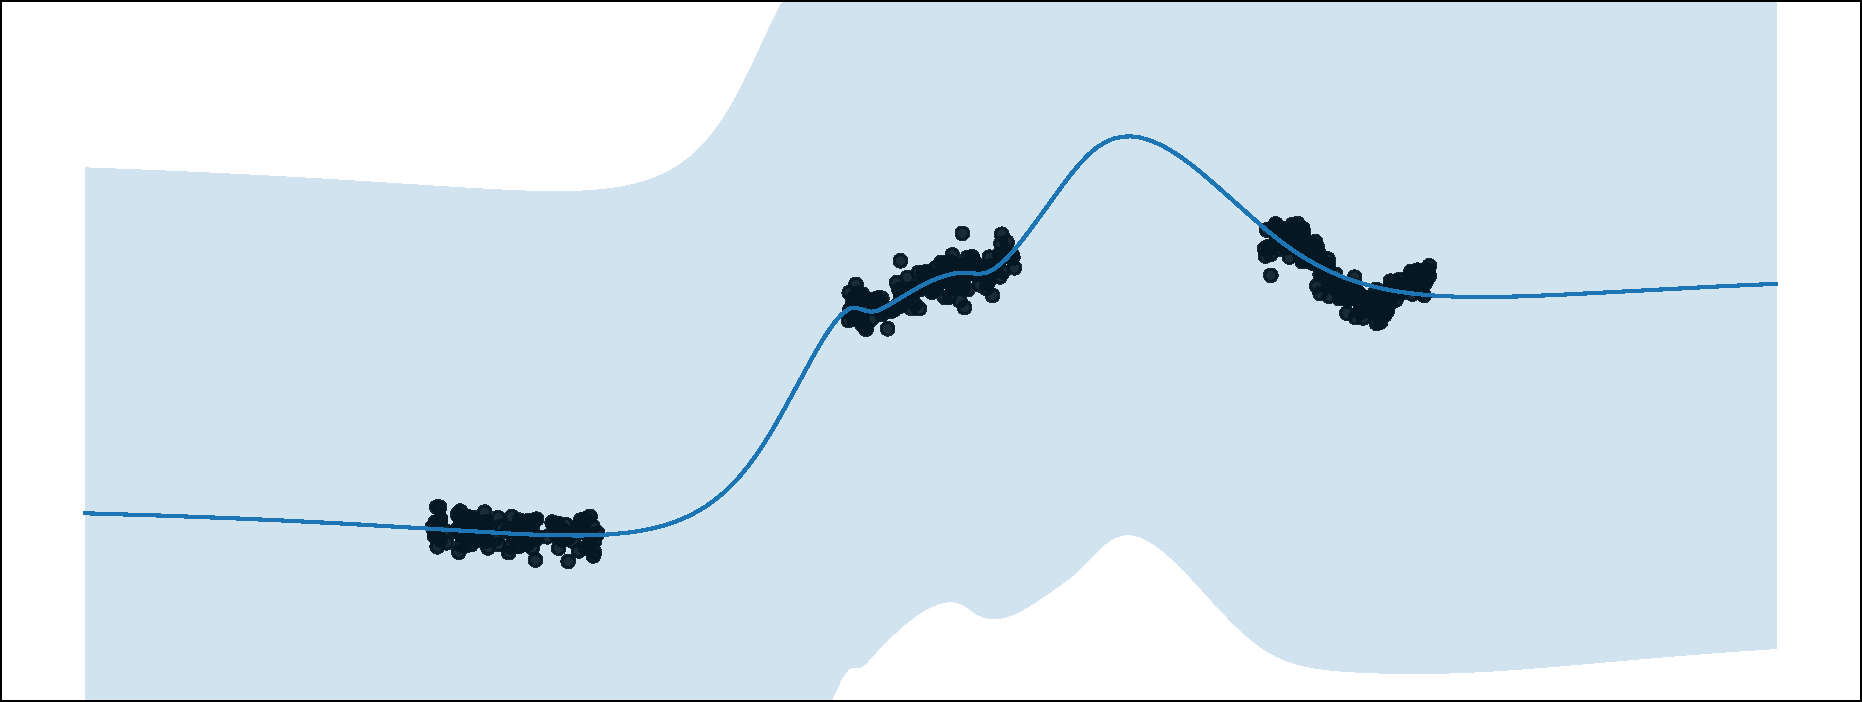
\includegraphics[width=0.30\textwidth]{imgs/Diag-LLA.pdf} & 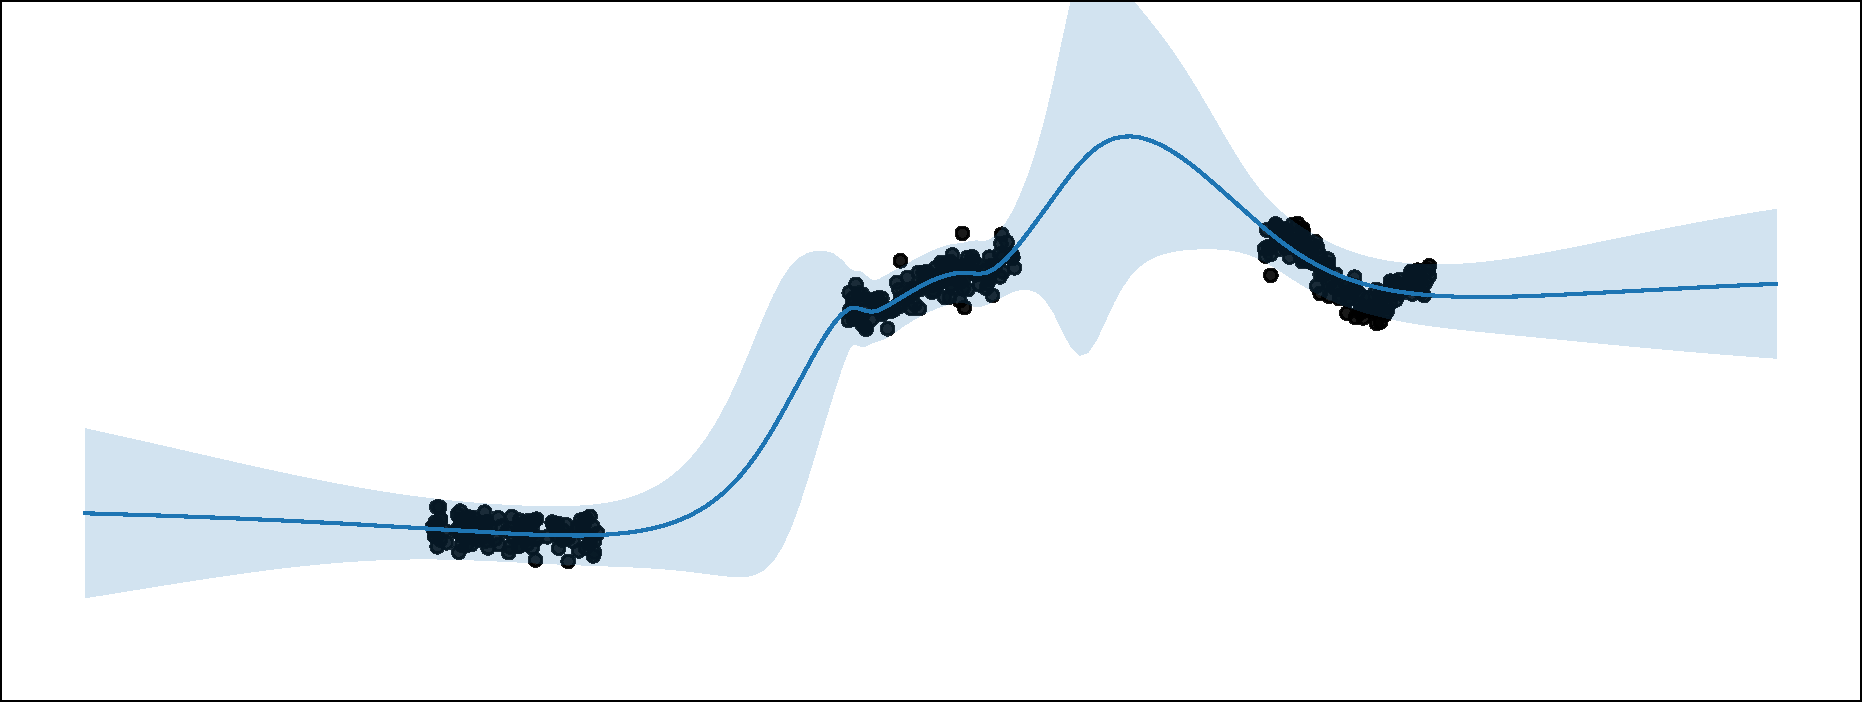
\includegraphics[width=0.30\textwidth]{imgs/LLA-KFAC.pdf} \\
        	\end{tabular}
        	\end{center}
            \caption{Predictive distribution (two times the standard deviation) on a toy 1D regression dataset with a 2 hidden layer MLP with \(50\) units.}
            \label{fig:intro}
        \end{figure}

    \end{frame}
    
    \begin{frame}
        \begin{figure}
        	\begin{center}
        	\begin{tabular}{cc}
            {\scriptsize VaLLA \(M = 10\)} & {\scriptsize ELLA \(M = 10\)} \\
        	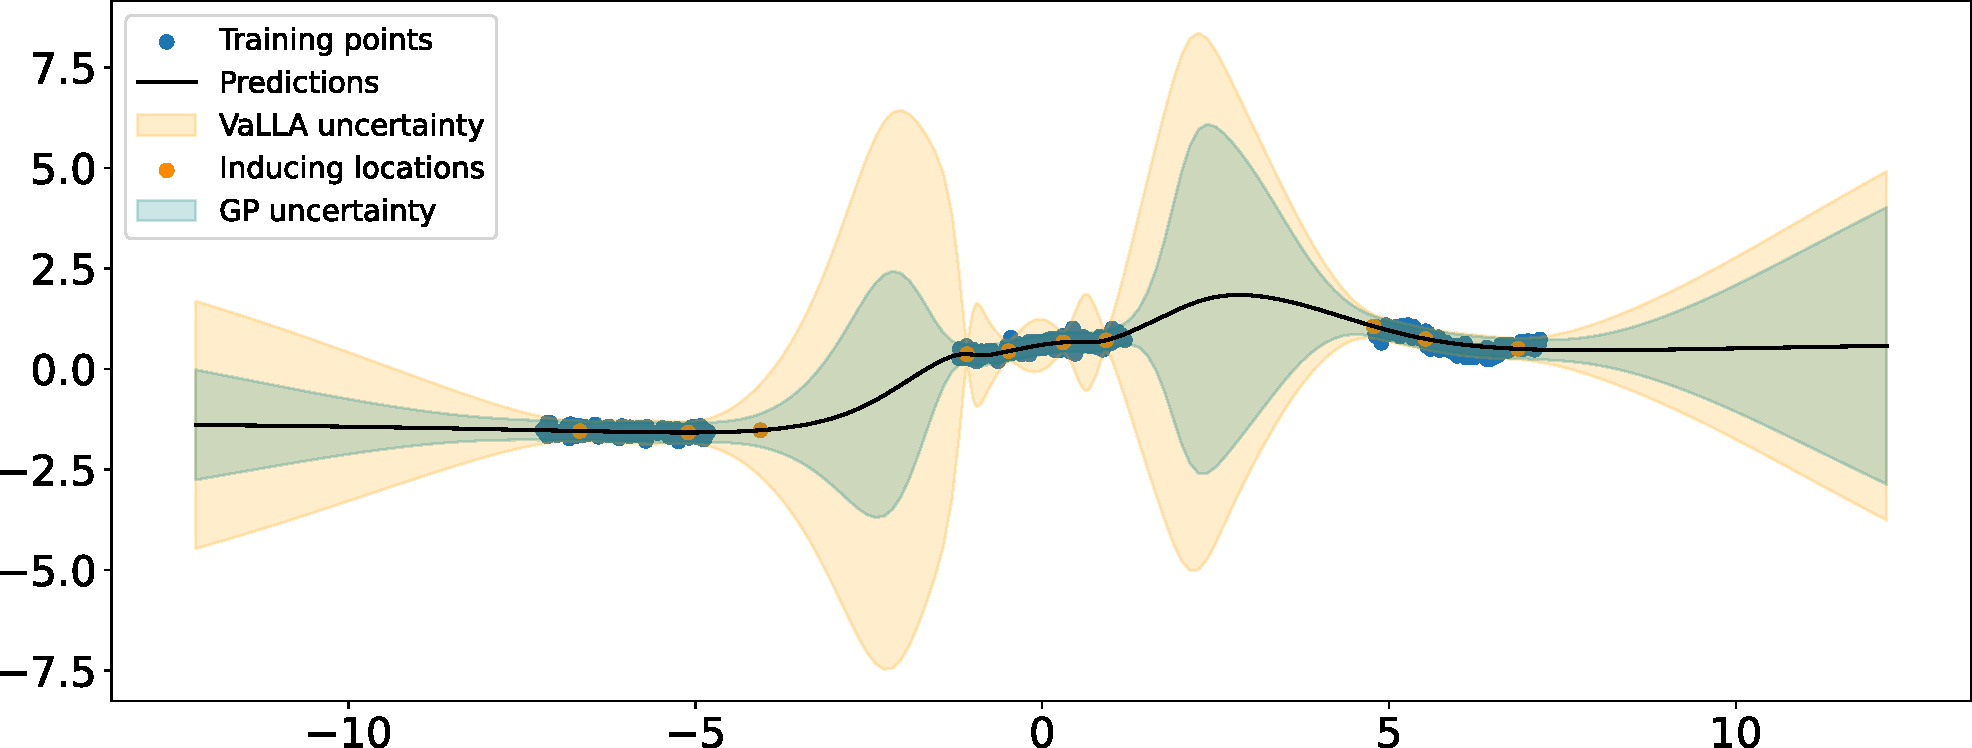
\includegraphics[width=0.45\textwidth]{imgs/SparseLA_M=10.pdf} & 
            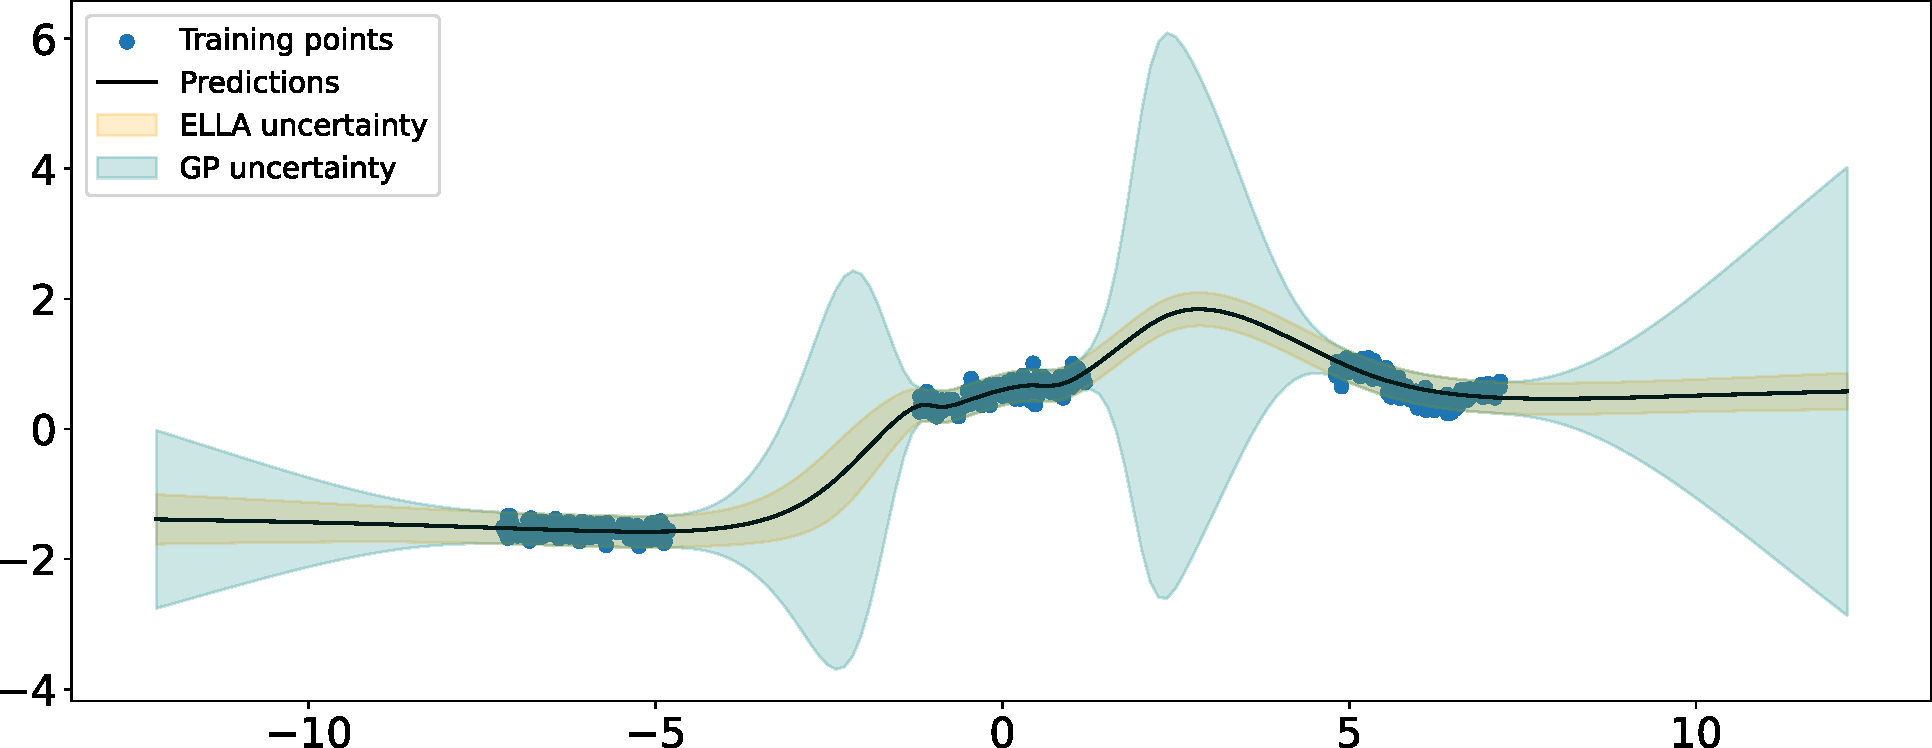
\includegraphics[width=0.45\textwidth]{imgs/ELLA_synthetic2_M=10.pdf} \\
            {\scriptsize VaLLA \(M = 20\)} & {\scriptsize ELLA \(M = 20\)} \\
            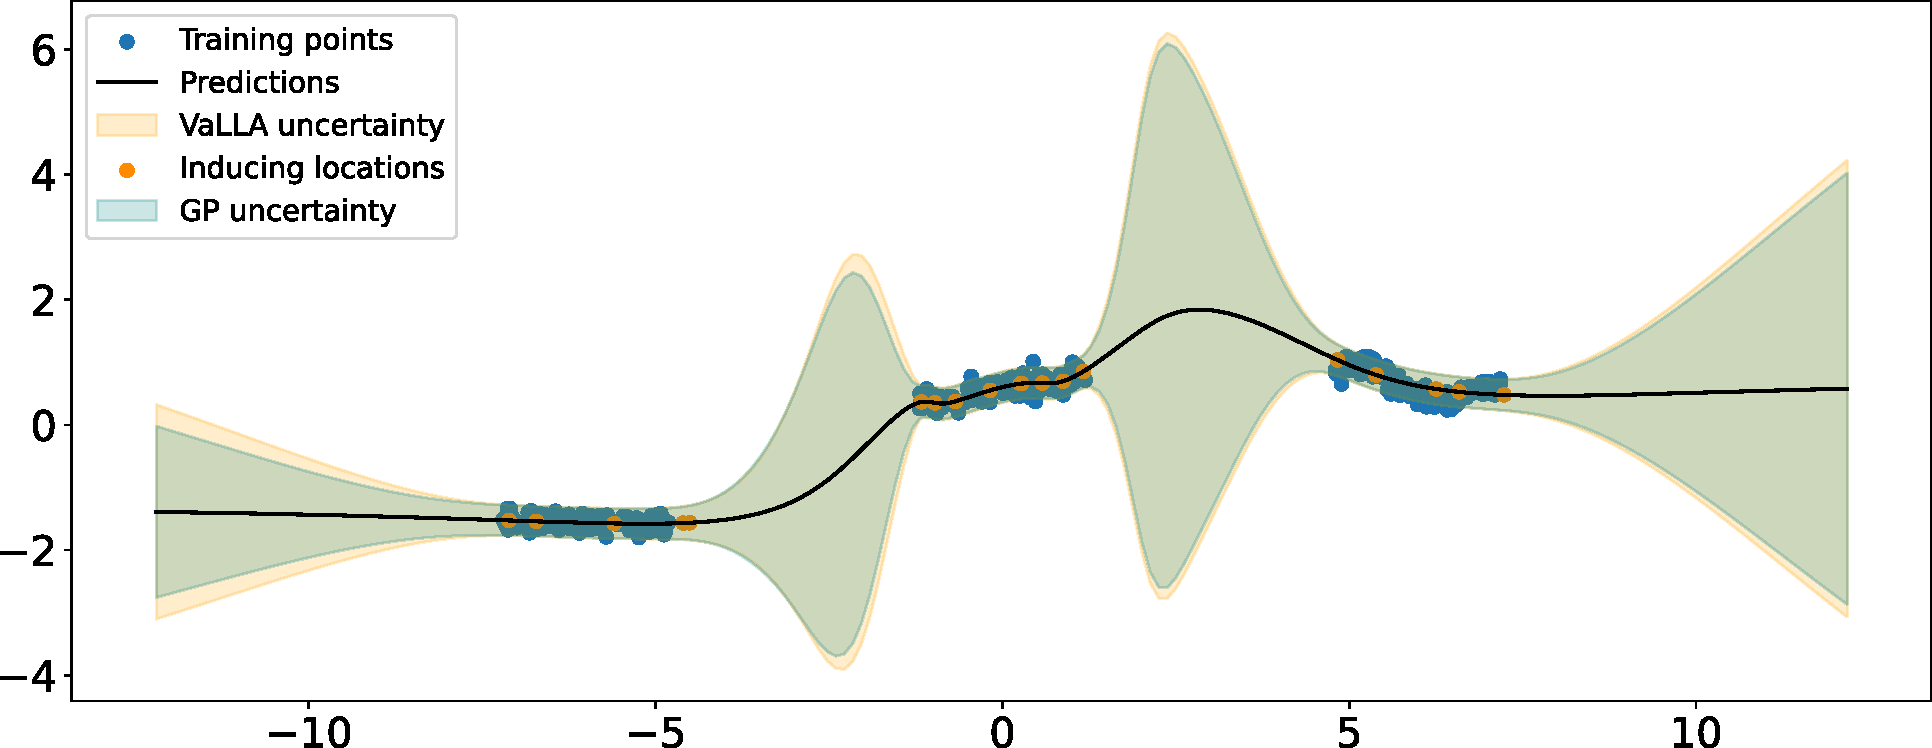
\includegraphics[width=0.45\textwidth]{imgs/SparseLA_M=20.pdf} & 
            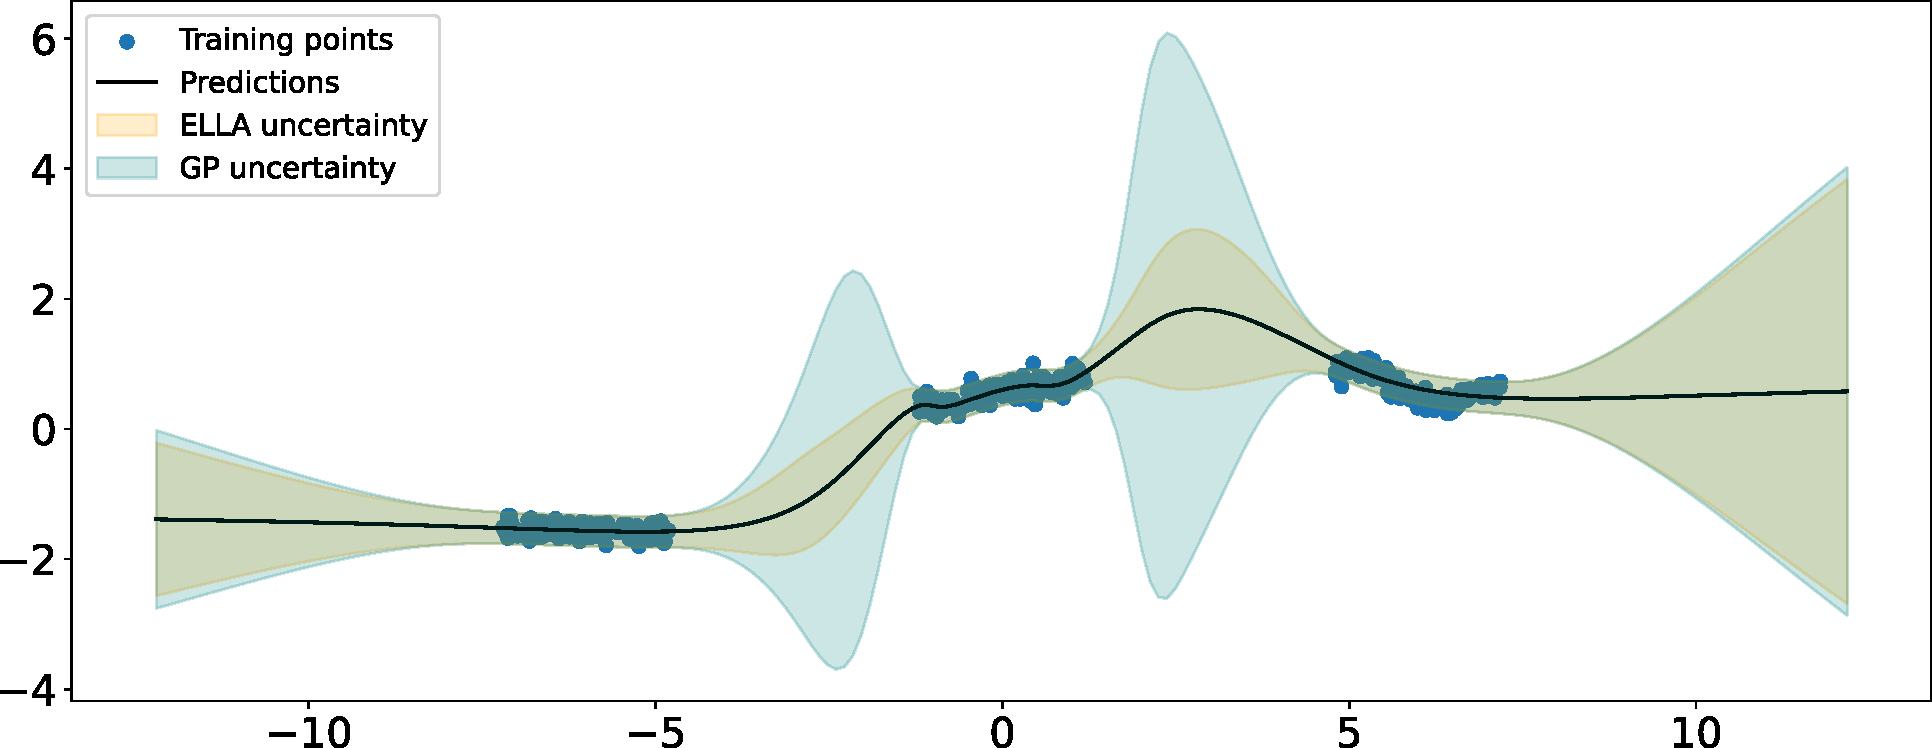
\includegraphics[width=0.45\textwidth]{imgs/ELLA_synthetic2_M=20.pdf} \\
            {\scriptsize VaLLA \(M = 30\)} & {\scriptsize ELLA \(M = 30\)} \\
            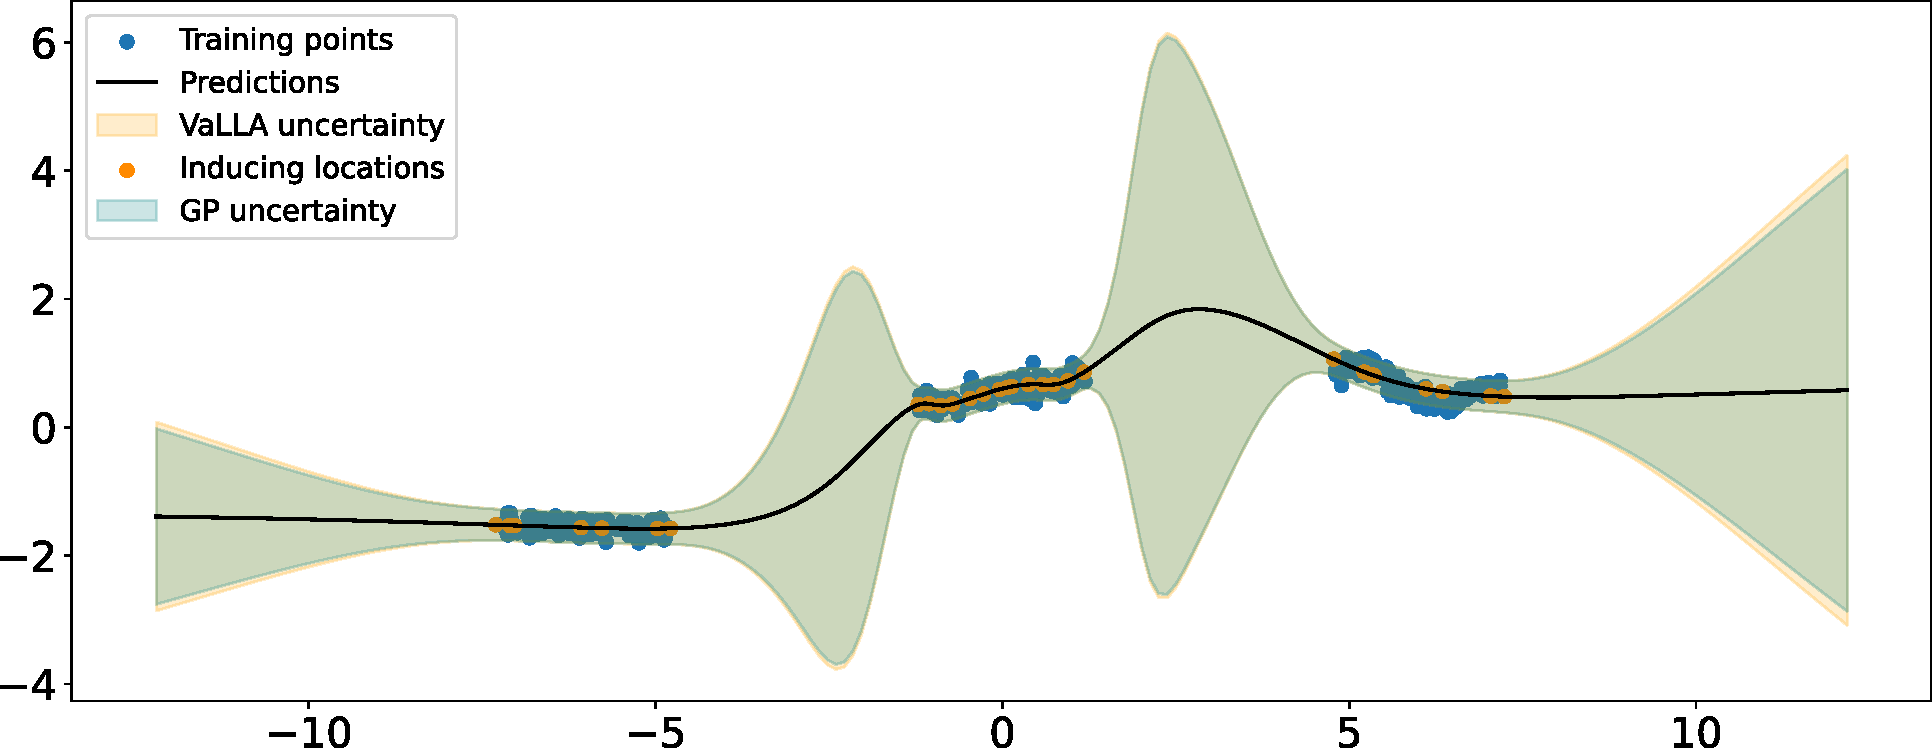
\includegraphics[width=0.45\textwidth]{imgs/SparseLA_M=30.pdf} &
            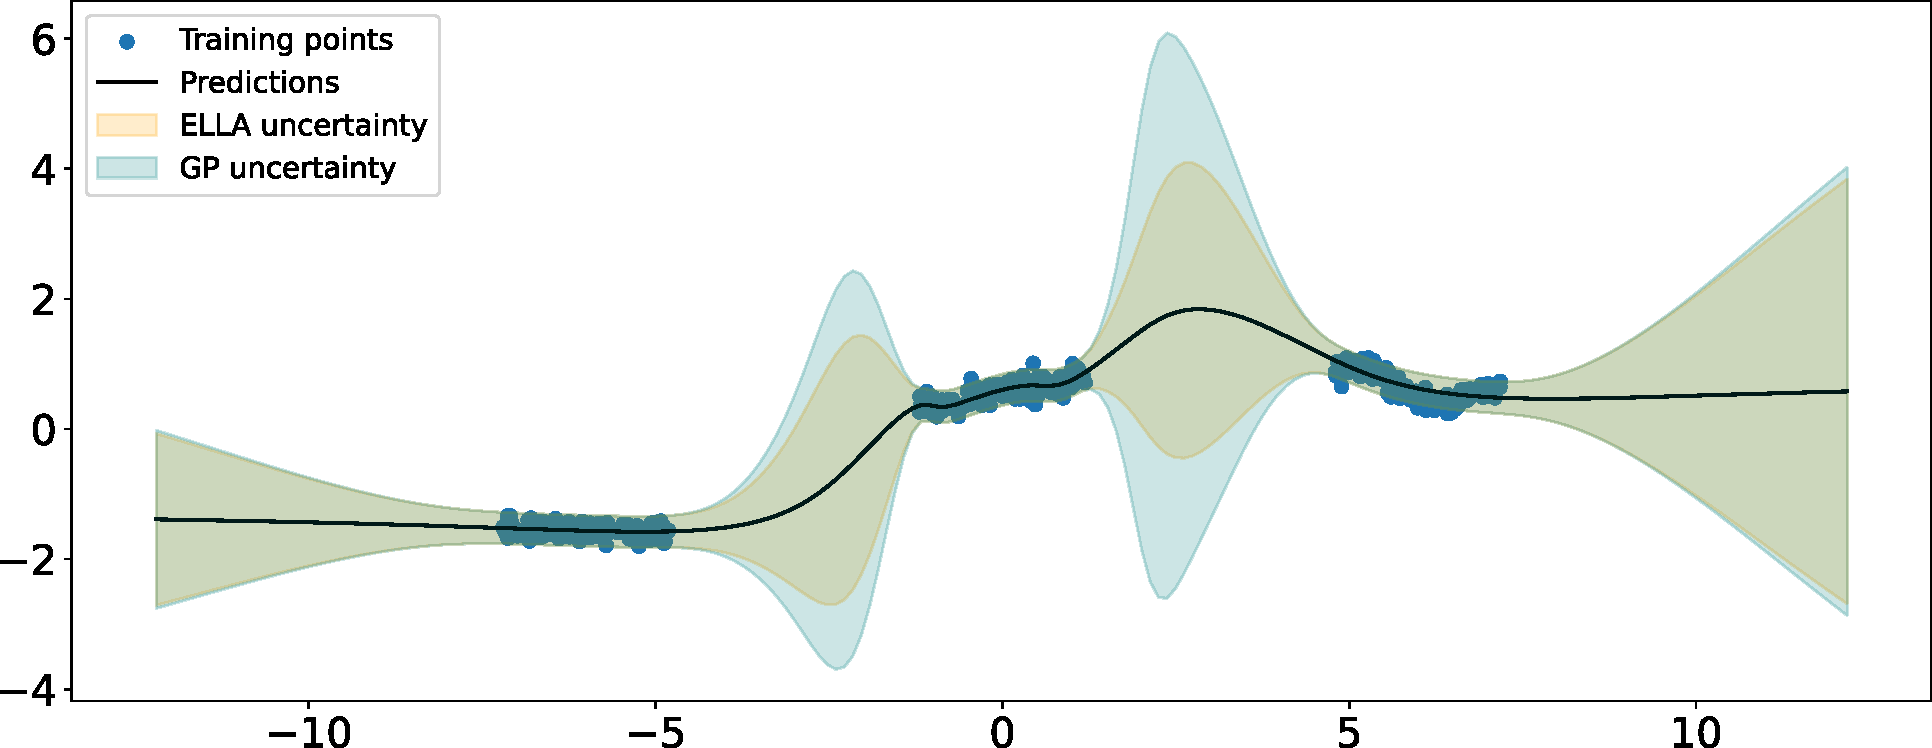
\includegraphics[width=0.45\textwidth]{imgs/ELLA_synthetic2_M=30.pdf} 
        	\end{tabular}
        	\end{center}
        \end{figure}
    \end{frame}


    \begin{frame}{Conclusions}
        \begin{enumerate}[<+->]
            \item Using the dual definition in RKHS, sparse GPs can be generalized to decouple the inducing points.
            \item The decoupled definition can be used to fix the mean of the GP to the pre-trained MAP solution.
            \item Stochastic optimization can be employed to train the model.
            \item As a result, VaLLA is scalable in both parameters and dataset size.
            \item The obtained preliminary results show competitive uncertainty estimation compared to other LLA approximations.
        \end{enumerate}
    \end{frame}

    \begin{frame}[standout]
        Thank you for your attention!
    \end{frame}

\begin{frame}[allowframebreaks]
\nocite{*}
\printbibliography[heading=none]
\end{frame}
\end{document}